\documentclass[report,10.5pt,oneside,openany,a4paper]{jsbook}
\pagenumbering{arabic}

\usepackage[top=30truemm, bottom=30truemm, left=30truemm, right=20truemm]{geometry}

\usepackage{amsmath,amssymb}
\usepackage{mathtools}
\usepackage{bm}
\usepackage[dvipdfmx]{graphicx}
\usepackage{subfigure}
\usepackage{verbatim}
\usepackage{wrapfig}
\usepackage{ascmac}
\usepackage{makeidx}
\usepackage{url}
\usepackage{times}

\usepackage{titlesec}
\usepackage{picture}
\usepackage[dvipdfmx]{color}
\usepackage[cc]{titlepic}

\usepackage[dvipdfmx]{hyperref}
\usepackage{pxjahyper}

\usepackage{afterpage}

% colors
\definecolor{teal}{RGB}{0,128,128}
\definecolor{powderblue}{RGB}{176,224,230}
\definecolor{darkslateblue}{RGB}{72,61,139}
\definecolor{darkslategray}{RGB}{47,79,79}
\definecolor{lightcyan}{RGB}{224,255,255}

% chapter
\titleformat{\chapter}[block]{\bfseries\Huge}{第 \thechapter 章}{0.5em}{}
\titlespacing{\chapter}{0pt}{0pt}{24pt}

% section
\titleformat{\section}[block]{\bfseries\huge}{\thesection}{0.5em}{}
\titlespacing{\section}{0pt}{24pt}{12pt}

% subsection
\titleformat{\subsection}[block]{\bfseries\Large}{\thesubsection}{0.5em}{}
\titlespacing{\subsection}{0pt}{24pt}{12pt}

\makeindex

\setlength{\baselineskip}{18pt}
\setlength{\textwidth}{\fullwidth}
\setlength{\textheight}{40\baselineskip}
\addtolength{\textheight}{\topskip}
\setlength{\voffset}{-0.55in}

\begin{document}

%タイトル開始

\begin{titlepage}
  \begin{center}
  \vspace*{50truept}
  {\Huge ブルーベリー栽培支援de}\\ % タイトル
  \vspace{10truept}
  % {\Large }\\ % サブタイトル
  \vspace{20truept}
  {\Huge  江﨑郁磨\ }\\ % 名前
  \vspace{10truept}
  {\Large Esaki Ikuma}\\ %ローマ字名
  \vspace{20truept}
  {\normalsize (20xx年度入学, xxxxxxxx)}\\ % 学籍番号
  \vspace{40truept}
  \vspace{40truept}
  {\huge 指導教員: 清水郁子 准教授 \ }\\ % 指導教員名
  \vspace{10truept}
  {\normalsize 東京農工大学 工学部 知能情報工学科}\\
  \vspace{10truept}
  {\normalsize 20xx 年度卒業論文}\\
  \vspace{10truept}
  {\normalsize (20xx年 x月 xx日 提出)}\\ % 提出日
  \end{center}
\end{titlepage}

\begin{titlepage}
  \newgeometry{left=20mm,right=20mm,bottom=30mm}
\begin{center}
{\normalsize 東京農工大学 工学部 知能情報システム工学科 20xx年度 卒業論文 要旨}\\
{\normalsize 題目 \ }
{\large ここに題目を書く}\\
{\normalsize You write your title here in English}\\
{\normalsize If your title is long, you write it here too.}\\
{\normalsize 学籍番号 00000000 \hspace{20pt}}
{\normalsize 氏名 自分野名前(Namae JIBUNNO)}\\
{\normalsize 提出日 20xx年 x月 x日}\\
\end{center}

ここに概要を書く.2000文字くらいで1ページ分.
概要には「背景」,「先行研究」,「目的」,「提案手法の内容」,「結果」を書く.
図は含めず,文章のみで説明する.

\restoregeometry
\end{titlepage}

%タイトル終わり
\frontmatter

\tableofcontents
\listoffigures
\listoftables


\mainmatter


\chapter{はじめに} % 章
\label{sec:はじめに}
\section{研究の背景}  % 節
\label{sec:研究の背景}

\section{本論文の構成}
\label{sec:本論文の構成}


\chapter{先行研究}\label{sec:RecentWorks}
本章では,先行研究で広く用いられるVision Transformer(ViT)について示したのち,それを用いたいくつかの先行研究を示す.

%%%%
\section{Vision Transformer}\label{sec:ViT}

研究の背景でもある Vision Transformer (ViT) \cite{Dosovitskiy_2021} は,
画像のクラス分類問題解決のために実装されたモデルである. 
モデルの設計は図 \ref{fig:vit_design} に示すとおりであり, 
Transformer Encoder \cite{Vaswani_2017} に BERT \cite{Devlin_2019} を適用した
``Transformer'' に加えて, 画像のトークン化を行う ``Tokenizer'' を構成要素に持つ. 
\begin{figure}[htbp]
  \centering
  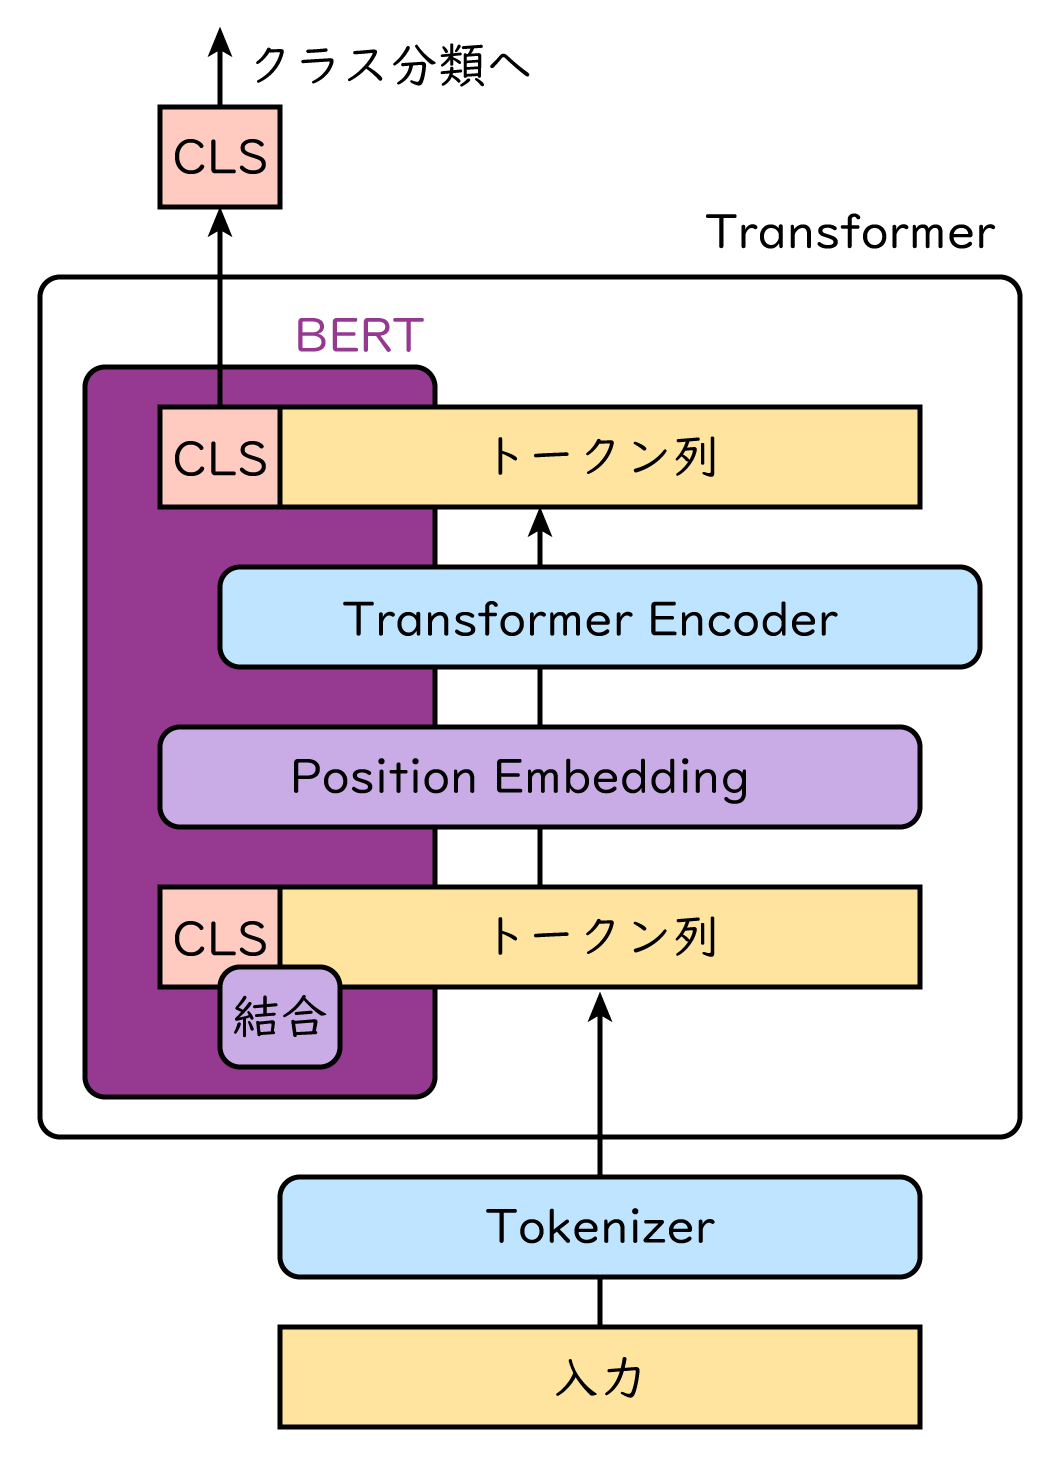
\includegraphics[width=.4\textwidth]{figure/vit_design.png}
  \caption{Vision Transformer の構成}
  \label{fig:vit_design}
\end{figure}

中略

%%%%
\subsection{BERT}\label{sec:bert}
BERT \cite{Devlin_2019} とは Bidirectional Encoder Representations from
Transformer の短縮表現であり, 自然言語処理領域にて発表されたモデルである.
ViT と同様, Transformer Encoder を基にしたモデルであり,
ViT の設計においても, BERTの要素技術が反映されている.

まず, ViTモデルのネットワーク規模は BERT の表現を踏まえたものとなっている.
具体的には, トークンの次元と Encoder Block の数, 次節で述べる MSA のヘッド数が
表 \ref{table:vit-netsize} のとおり定められている. 
ViT では Base(B) のネットワーク規模であることを, ViT-B と表記することで明示している. 
\begin{table}[htbp]
  \caption{ViT(BERT)のネットワーク規模}
  \label{table:vit-netsize}
  \centering
  \begin{tabular}{l|lccc}
    \hline
    ネットワーク規模 & ViTの表記 & トークンの次元($d_{t}$) & Encoder Block の数 
    & MSA のヘッド数 \\\hline\hline
    Base(B) & ViT-B & 768 & 12 & 12 \\
    Large(L) & ViT-L & 1024 & 24 & 16 \\
    \hline
  \end{tabular}
\end{table}

中略

%%%%
\subsection{計算量}\label{sec:calc}

トークン数 $l$ とその次元 $d_{t}$ による影響を明確にするため, 
$T \lparen d_{vec} \rparen$ は変数を用いた表現へと改める. 
内積における計算処理が, 要素積に対して総和を求めていることを考慮すると 
時間計算量 $T \lparen d_{vec} \rparen$ は $d_{vec}$ の比例関数とみなせるため, 
$\alpha d_{vec} + \beta$ によって近似する. 
加えて, ViT-B16においては, $d_{t}=hd_{m}=768$ かつ $l=256$ であるため, 
$ld_{t}$ および $l^{2}h$ は $ld_{t}^{2}$ や $l^{2}d_{t}$ に対して, 十分小さいものとする. 
以上から, 全体の時間計算量 $T_{msa}$ は式 \eqref{eq:cp_timesub} のとおり推定する.
時間計算量の推定値において, トークン数 $l$ による時間計算量のオーダーは 
$O \lparen n^{2} \rparen$ であり, トークン数の増加は実行時間に大きく影響することが分かる. 
\begin{align}
  \label{eq:cp_timesub}
  T_{msa} &= 3 l d_{t} \lparen \alpha d_{t} + \beta \rparen + l d_{t} \lparen \alpha d_{t} + \beta \rparen 
  + l^{2} h \lparen \alpha d_{m} + \beta \rparen + l d_{t} \lparen \alpha l + \beta \rparen \nonumber\\
  &= 2 l d_{t} \lparen 2 d_{t} + l \rparen \alpha  
\end{align} 

\chapter*{謝辞} \label{sec:Acknowledgments}

本論文を執筆するにあたり,清水郁子教授には指導教員として終始熱心なご指導を頂きました.心から感謝いたします.
また,~~.
最後に,一緒に研究に取り組み,多くの助言や激励をいただいた研究室の皆様に感謝を申し上げます.


\appendix
\chapter{補足} % 本文の補足

\clearpage
\newpage
\begin{thebibliography}{9}
  \bibitem[Krizhevsky et al. 2012]{Krizhevsky_2012}
  Krizhevsky Alex, Sutskever Ilya, and Hinton Geoffrey E.
  Imagenet classification with deep convolutional neural networks.
  In Advances in neural information processing systems,
  volume 25, pages 1097--1105, 2012.
  \bibitem[Radford et al. 2015]{Radford_2015}
  Radford Alec, Metz Luke, and Chintala Soumith.
  Unsupervised Representation Learning with Deep Convolutional 
  Generative Adversarial Networks. In ICLR, 2016.
  \bibitem[He et al. 2016]{He_2016}
  He Kaiming, Zhang Xiangyu, Ren Shaoqing, and Sun Jian
  Deep residual learning for image recognition.
  In Proceedings of the IEEE conference on computer vision and pattern recognition,
  pages 770--778, 2016.
  \bibitem[Zhang et al. 2019]{Zhang_2019}
  Zhang Han, Goodfellow Ian, Metaxas Dimitris, and Odena Augustus.
  Self-attention generative adversarial networks.
  In International conference on machine learning, pages 7354--7363, PMLR.
  \bibitem[Vaswani et al. 2017]{Vaswani_2017}
  Vaswani Ashish, Shazeer Noam, Parmar Niki, Uszkoreit Jakob, Jones Llion, 
  Gomez Aidan N, Kaiser, {\L}ukasz, and Polosukhin Illia.
  Attention is all you need.
  In Advances in Neural Information Processing Systems, pages 5998-6008, 2017.
  \bibitem[Wang et al. 2018]{Wang_2018}
  Wang Xiaolong, Girshick Ross, Gupta Abhinav, and He Kaiming.
  Non-local neural networks.
  In Proceedings of the IEEE conference on computer vision and pattern recognition,
  pages 7794--7803, 2018.
  \bibitem[Parmar et al. 2018]{Parmar_2018} Parmar Niki, Vaswani Ashish,
  Uszkoreit Jakob, Kaiser Lukasz, Shazeer Noam, Ku Alexander, and Tran Dustin.
  Image Transformer.
  In Proceedings of the 35th International Conference on Machine Learning,
  pages 4055--4064. PMLR, Jul, 2018.
  \bibitem[Child et al. 2019]{Child_2019} Child Rewon, Gray Scott, Radford Alec, 
  and Sutskever Ilya.
  Generating Long Sequences with Sparse Transformers. 
  In CoRR, May, 2019.
  \bibitem[Dosovitskiy et al. 2021]{Dosovitskiy_2021}
  Dosovitskiy Alexey, Beyer Lucas, Kolesnikov Alexander, Weissenborn Dirk, Zhai Xiaohua, 
  Unterthiner Thomas, Dehghani Mostafa, Minderer Matthias, Heigold Georg, Gelly Sylvain, 
  Uszkoreit Jakob, and Houlsby Neil.
  An Image is Worth 16x16 Words: Transformers for Image Recognition at Scale
  In International Conference on Learning Representations, 2021
  \bibitem[Olga et al. 2015]{Olga_2015}
  Olga Russakovsky, Jia Deng, Hao Su, Jonathan Krause, Sanjeev Satheesh, Sean Ma,
  Zhiheng Huang, Andrej Karpathy, Aditya Khosla, Michael Bernstein, Alexander C. Berg, 
  and Li Fei-Fei.
  ImageNet Large Scale Visual Recognition Challenge.
  In International Journal of Computer Vision (IJCV) 3, volume 3, pages 4171--4186, 2015.
  \bibitem[Devlin et al. 2019]{Devlin_2019}
  Devlin Jacob, Chang Ming-Wei, Lee Kenton, and Toutanova Kristina.
  BERT: Pre-training of Deep Bidirectional Transformers for Language Understanding.
  In Proceedings of the 2019 Conference of the North American Chapter
  of the Association for Computational Linguistics: Human Language Technologies,
  volume 1, pages 4171--4186, Jun, 2019.
  \bibitem[Wu et al. 2020]{Wu_2020}
  Wu Bichen, Xu Chenfeng, Dai Xiaoliang, Wan Alvin, Zhang Peizhao, Tomizuka Masayoshi,
  Keutzer Kurt, and Vajda P{\'e}ter
  In ArXiv, volume abs/2006.03677, 2020.
  volume={abs/2006.03677}
  \bibitem[Yuan et at. 2021]{Yuan_2021}
  Yuan Li, Chen Yunpeng, Wang Tao, Yu Weihao, Shi Yujun, Jiang Zi-Hang, Tay Francis E.H., 
  Feng Jiashi, and Yan Shuicheng.
  Tokens-to-Token ViT: Training Vision Transformers From Scratch on ImageNet.
  In Proceedings of the IEEE/CVF International Conference on Computer Vision (ICCV),
  pages 558--567, October, 2021.
  \bibitem[Kingma and Ba. 2015]{Kingma_Ba_2015}
  Diederik P. Kingma and Jimmy Ba.
  Adam: {A} Method for Stochastic Optimization.
  In 3rd International Conference on Learning Representations, {ICLR}, May, 2015.
\end{thebibliography}



\newpage
\printindex

\end{document}
